%%%%%%%%%%%%%%%%%%%%%%%%%%%%%%  IEEEsample.tex
%%%%%%%%%%%%%%%%%%%%%%%%%%%%%%%%%%%%%%%%%
%%%%%%%%%%%%%%%%%%%%%%%    More information: see the header of IEEEtran.sty
%%%%%%%%%%%%%%%%%%%%%%%
%%%%%%%%%%%%%%%%%%%%%%%%%%%%%%%%%%%%%%%%%%%%%%%%%%%%%%%%%%%%%%%%%%%%%%%%%%%%%%%%
%%%%

\documentclass{llncs}

\usepackage{helvet}
\usepackage{enumerate}
\usepackage{amsmath}
\usepackage{amsfonts}
\usepackage{graphicx}
\usepackage{multirow}
\usepackage{subfig}
\RequirePackage{algorithmic}
\RequirePackage{algorithm}


\input{epsf}
\def\BibTeX{{\rm B\kern-.05em{\sc i\kern-.025em b}\kern-.08em1
    T\kern-.1667em\lower.7ex\hbox{E}\kern-.125emX}}

%\newtheorem{Definition}{definition}[section]
%\newtheorem{example}{Example}
%\newtheorem{Lemma}{Lemma}

% New command for the table notes.
\def\tabnote#1{{\small{#1}}}

% New command for the line spacing.
\newcommand{\ls}[1]
    {\dimen0=\fontdimen6\the\font
     \lineskip=#1\dimen0
     \advance\lineskip.5\fontdimen5\the\font
     \advance\lineskip-\dimen0
     \lineskiplimit=.9\lineskip
     \baselineskip=\lineskip
     \advance\baselineskip\dimen0
     \normallineskip\lineskip
     \normallineskiplimit\lineskiplimit
     \normalbaselineskip\baselineskip
     \ignorespaces
    }

\newcommand{\beq}{\begin{equation}}
\newcommand{\eeq}{\end{equation}}
\newcommand{\ov}{\overline}
%\newcommand{\ov}{\bar}
\newcommand{\xor}{\bigoplus}
%%
%\newtheorem{algorithm}{Algorithm}[section]

\newcommand{\Fq}{{\mathbb{F}}_{q}}
\newcommand{\Fkk}{{\mathbb{F}}_{2^k}}
\newcommand{\Fkkx}[1][x]{\ensuremath{\mathbb{F}}_{2^k}[#1]\xspace}
\newcommand{\Grobner}{Gr\"{o}bner\xspace}
\newcommand{\B}{{\mathbb{B}}}
\newcommand{\F}{{\mathcal{F}}}
\newcommand{\G}{{\mathcal{G}}}
%%%

\newcommand{\debug}[1]{\textcolor{gray}{[ #1 ]}}


\begin{document}

\title{{Deriving Canonical Polynomial Representations from Circuits using Gr\"obner Bases}}

\author{
T. Pruss\inst{1} \and P. Kalla\inst{1} \and F. Enescu\inst{2}
}

\institute{
Electrical \& Computer Engineering\\
University of Utah, USA
\and
Mathematics \& Statistics\\
Georgia State University, USA
}

\maketitle

%\thispagestyle{empty}
%\pagestyle{empty}

\begin{center}{\bf ABSTRACT}\end{center}
Sequential equivalence and model checking techniques are widely
employed in hardware and software verification. With the increasing
size and complexity of hardware/software systems, abstraction has
become a key component to address scalability.
This dissertation investigates new abstraction techniques at word-level and their applications 
on sequential circuits verification. By bundling together $k$ bit-level state-variables into
one word-level constraint expression, the state-space can be construed
as a polynomial function over the finite (Galois) field of $2^k$
elements. As long as the state-space are modeled as polynomial ideals
over word-level variables, algebraic geometry techniques including ideal manipulations,
Gr\"obner bases reasoning and finite field algebra are researched to 
facilitate new word-level abstractions.

Algebraic geometry offers a very powerful set of tools to reason about
the properties of the solutions to a system of polynomial
constraints. Moreover, the algebraic model inherently provides a
framework for abstraction. 
The algebraic geometry algorithms (Groebner basis computations) exhibit
high complexity which prevent it from being widely used in conventional techniques. 
Interestingly, recent experience has shown that
by analyzing the topology of circuits in conjunction with Gr\"obner
basis computations helps to identify the structure and symmetry
inherent in the problem, this lower the computational complexity.

Formal verification of sequential circuits requires the analysis of
the underlying finite state machine. Reachability analysis becomes a
fundamental tool for this purpose. We devised traditional traversal algorithms 
using the new abstraction method to perform
the reachability analysis at word-level. 
The abstractions are also exploited on functional
verification of sequential Galois field arithmetic circuits, where conventional 
techniques fail to provide scalability. At last, we propose a new method to extract 
unsatisfiable cores and utilize the information about the cores to 
perform model checking with abstraction refinement.
\chapter{Introduction}
\label{ch:intro}
\vspace{-0.8cm}
\section{Hardware Design and Verification Overview}
During the past decades, the level of integration in modern VLSI systems is becoming higher and higher because of the Moore's law.
As a result, an entire system with billions of transistors can be built upon a single chip.
The design process also evolves from manual design with little validation, to 
a formal 3-step procedure which requires collaboration of teams with large number of 
engineers. The 3 major steps are: 1) Design, which is to specify and enter the design intent;
2) Implement, which is to refine the design through various abstraction levels with the assistance of Computer-Aided-Design (CAD)
tools; 3) Verify, which is to verify the correctness of design and implementation.

Nowadays the verification step is usually completed by a team that specializes on test, verification and validation of 
circuits. This step is also automated as an indispensable part of the CAD flow, when circuit synthesis is performed. 
Figure \ref{fig:designflow} shows the typical synthesis flow, which covers procedures starting from the 
register-transfer-level (RTL) description (using hardware design languages, {\it i.e.} HDL) to  the 
physical design on silicon (depicted by the layout). The objective of verification in synthesis is 
to ensure the implementation is consistent with the original design intent. Verification is 
an important quality control measure before sending design layout to the VLSI foundries.
Considering the high cost of fabrication, faults and errors in the design will bring considerable 
waste of funds for the designers. On the other hand, all aspects of the society increasingly depend on 
the stability and accuracy of digital VLSI circuits; even small flaws or short-time failures can cause 
huge loss, especially in medical applications, military facilities and financial systems.
Therefore, it is of utmost importance to verify the correctness of VLSI designs.

One way to perform verification is by {\it simulation}. It is the collage of all circuit validation 
methods which apply stimulus on the inputs of circuit model and verify correctness of the outputs.
However, simulation is not a complete solution to circuit verification problems. In modern designs with 
large number of logic components and complicated architectures, it is impractical to simulate all possible 
test vectors. Usually only test vectors that correspond to typical failures are selected in simulation, which 
cannot cover unexpected failure patterns caused by special inputs. The notorious Intel FDIV bug \cite{nicely:FDIV}
is a good example where simulation failed. Failure occurred with input assignments which were rarely used in most divisions. Because of the limitation of simulation,  
test engineers from Intel failed to detect the bug,  which brought about $\$475$ million dollars recalling bill
for the company. Thus,  new methods that can guarantee the correctness of the design are necessary to be explored.

Another method developed besides simulation is \emph{formal verification}, it utilizes 
mathematical theory to reason about the correctness of hardware designs.
Formal verification can provide $100\%$ fault coverage from two aspects. On the one hand,  
it adopts formal languages to strictly describe the design intent and detailed implementation, 
and deduces circuit function from the implementation.
On the other hand,  it formalizes properties
for the circuit model which are relevant only to specific input signals,  and prove the properties mathematically. 
These descriptions are named as {\it specifications}.
Formal verification has two main forms: property checking and equivalence 
checking. 

\section{Formal Verification: Property and Equivalence Checking}
{\it Property checking} (or property verification) verifies
that a design satisfies certain given properties. Property checking is done mainly 
in the form of theorem proving (TP), model checking (MC), or TP/MC hybrid approaches.
\begin{enumerate}[{1)}]
\item \emph{Theorem proving} \cite{theoremproving:91} 
is a method of reasoning and mathematical logic dealing with proving 
mathematical theorems. In the application to circuit property checking, 
the specification as well as the circuit implementation
is described as theorems in mathematical logic. Subsequently logic rules
are employed to deduce new objective theorems. In practice, the tool can reduce
a proof goal to simpler sub-goals for automatic verification.

\item \emph{Model checking} \cite{modelcheck:99} is a technique 
for verifying if the specification properties are violated in finite-state systems. In the circuit verification 
domain, both the specification and the circuit implementation are modeled as a system of 
logic formulas. The finite-state system is then traversed to check if the 
properties are violated. If violation occurs, 
a counter-example is then generated as a transition firing path that corresponds to the
false behavior in the design. 
Modern model checking techniques use the error-trace to automatically refine
the system and perform further checking.
\end{enumerate}

{\it Equivalence Checking} verifies that two different representations of
a circuit design have equivalent functionality. It can be applied to 
multiple steps in the hardware design flow in Figure \ref{fig:designflow},
such as checking functional equivalence between HDL description and RTL,
checking RTL equivalence between RTL and synthesized/optimized netlist, 
and checking layout verification between netlist and layout for fabrication.

\begin{figure}[bp]
\centerline{
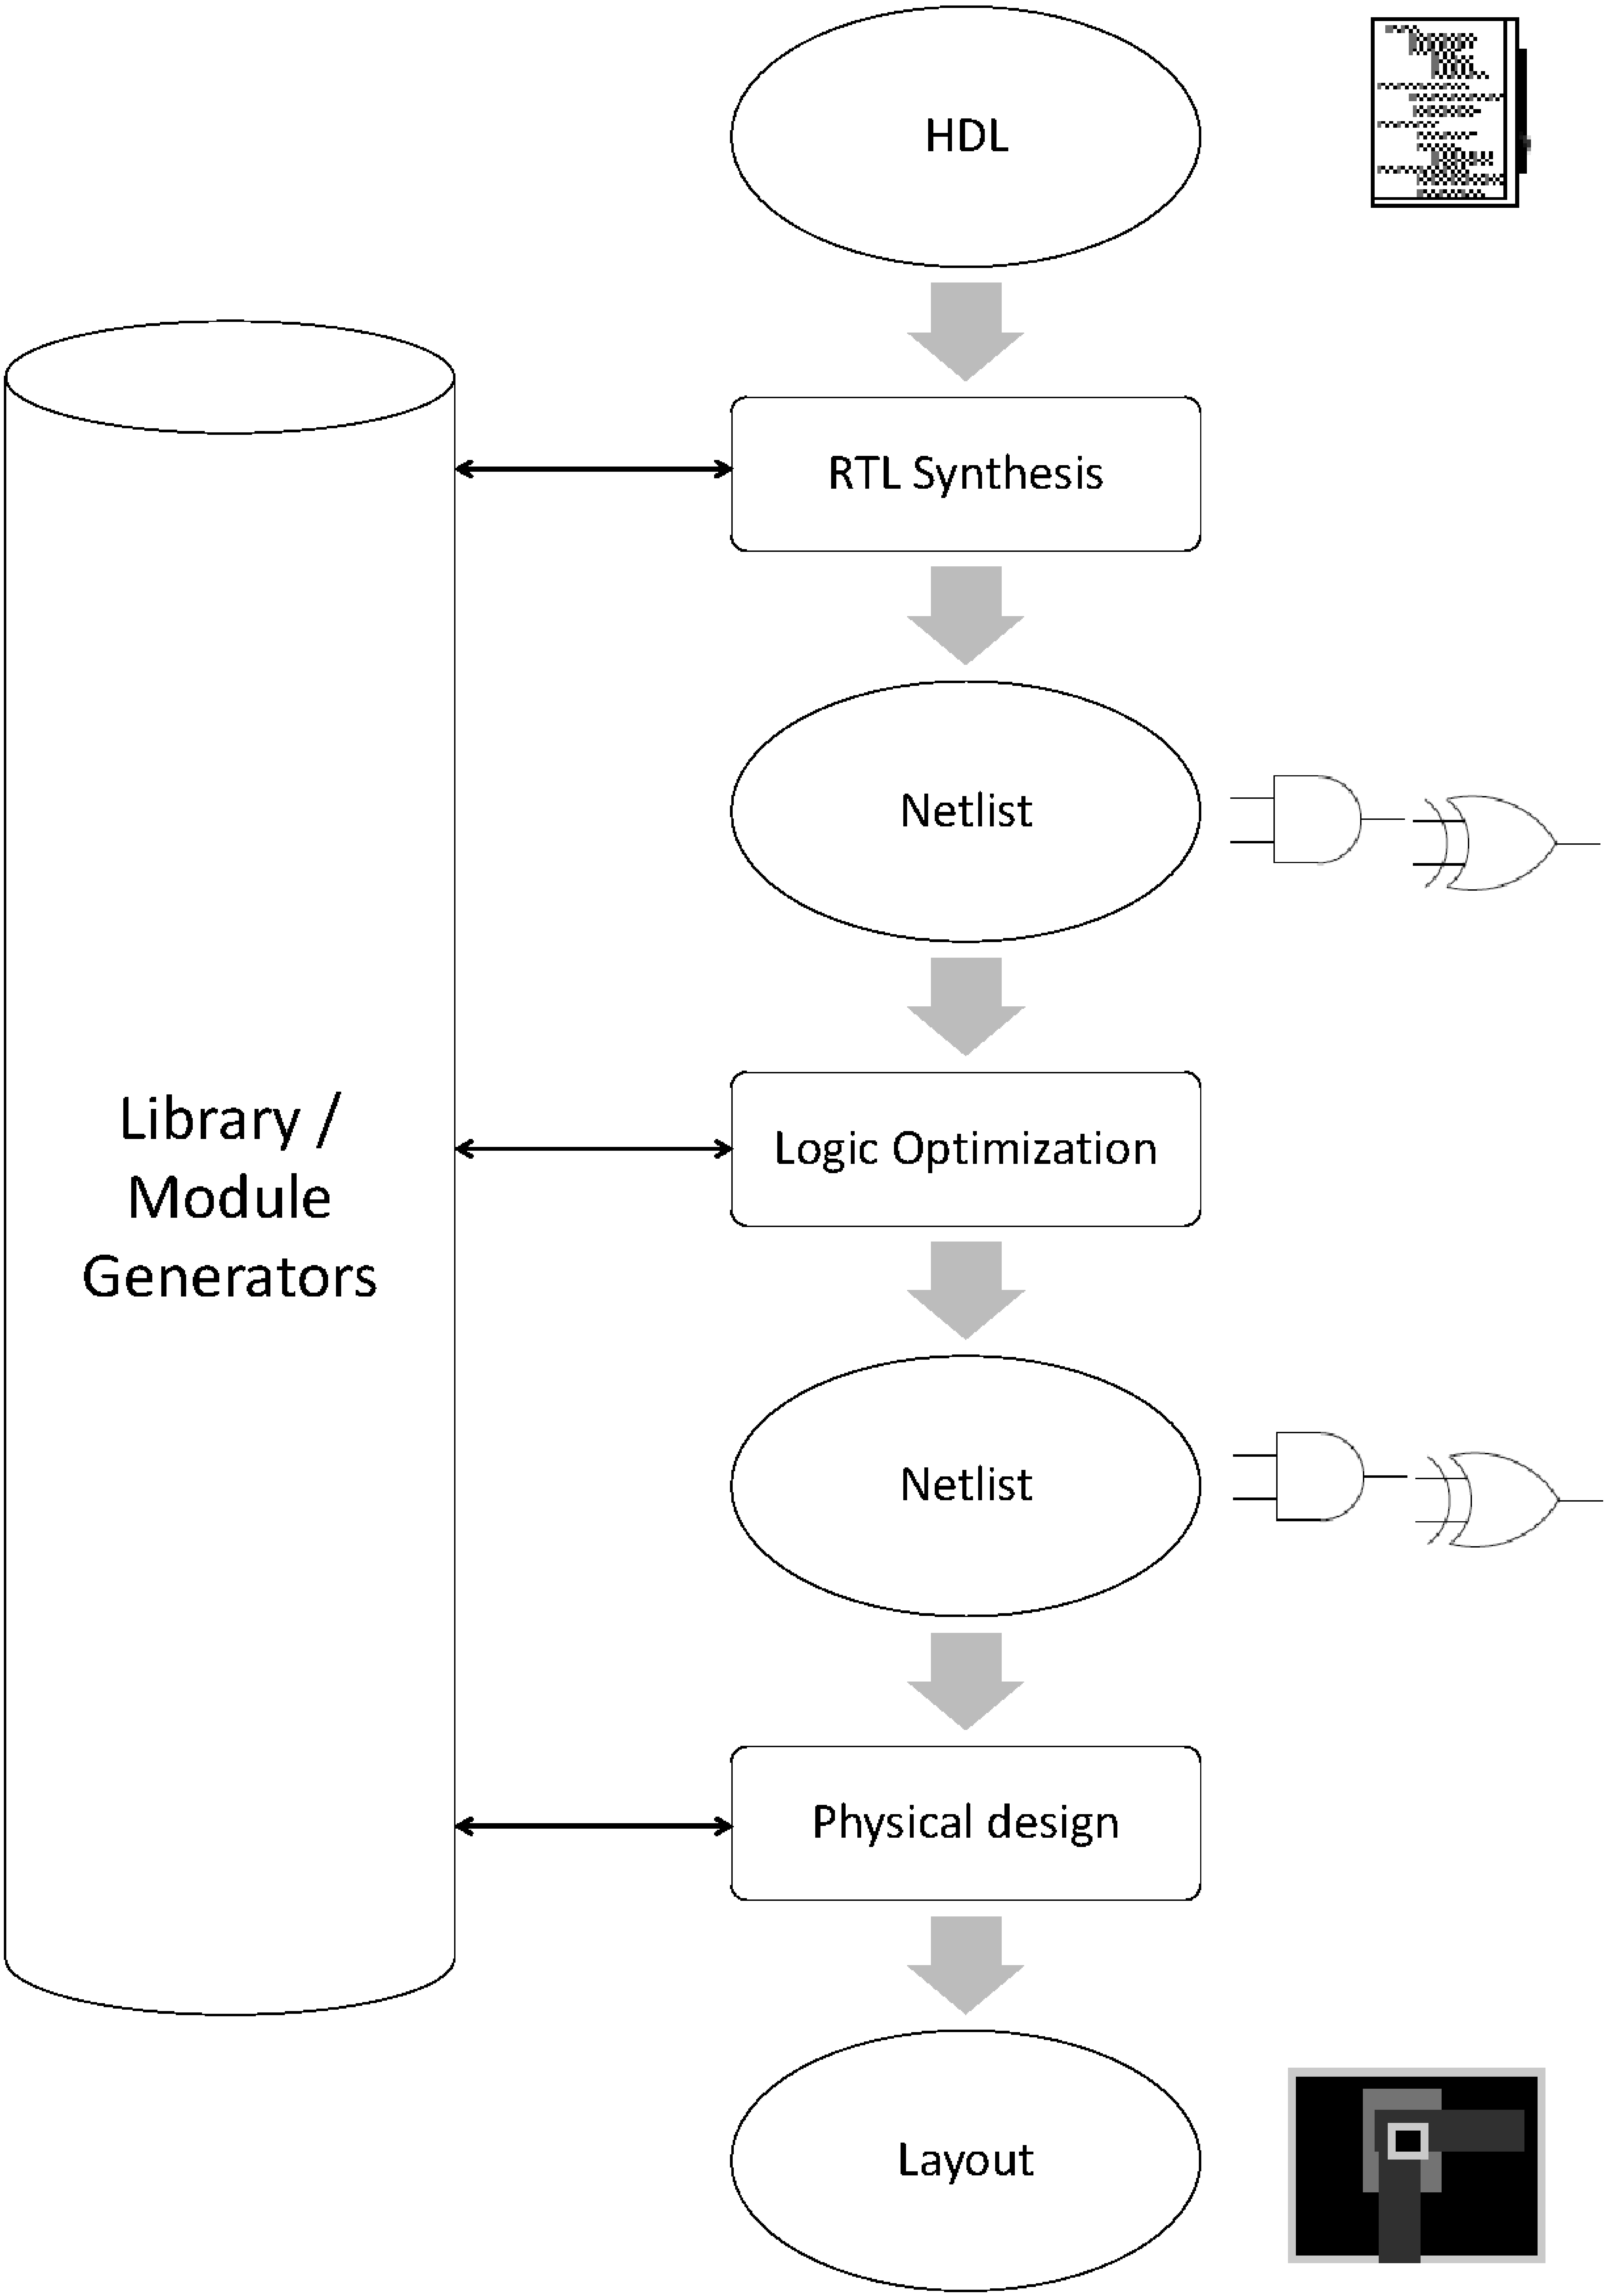
\includegraphics[width=0.7\textwidth]{newfig/designflow.eps}
}
\caption{Typical hardware design flow.}
\label{fig:designflow}
\end{figure}

There are three major
equivalence checking techniques: graph-based,
satisfiability-based (SAT-based) and induction-based.
\begin{enumerate}[{1)}]
\item \emph{Graph-based} techniques compare two circuit implementations 
by representing them using canonical graphs. 
The earliest invented canonical graph is the \emph{Binary Decision Diagram} (BDD) \cite{BRYA86}.
Many variants branch out from BDDs; some widely used variants include 
ZDD \cite{minato1993zero}, BMD \cite{bmd}, FDD \cite{okfdd}, {\it etc.} The comparison algorithms can 
determine whether the two graphs are isomorphic. The canonicity of the graph representation guarantees that
the graphs correspond to the two circuits will be 
equivalent if and only if the circuits implement the same function.
\item \emph{Satisfiability} (SAT) techniques utilize the satisfiability theory.
In circuit equivalence checking, a miter of the two circuits is created.
A \emph{miter} is a combination of the two circuits with one bit-level output, which 
gives output ``1" only when the outputs of the circuits differ with 
the same inputs, {\it e.g. }inputs $a,b,c$ shown in Figure \ref{fig:miter}. 
A SAT solver \cite{csat,mishchenko2006improvements} is then employed to simplify the problem 
and find a satisfying assignment to the inputs for which the 
miter output is ``1". If such an assignment exists, this solution acts as a 
counter-example to equivalence; otherwise the circuits
are functionally equivalent.
\item \emph{Induction-based} techniques are developed and applied to verify the 
equivalence between sequential circuits, which is called the {\it sequential equivalence checking}
(SEC) problem. A miter model can also be built with two sequential circuits. Through the 
miter model, SEC problem is transformed into a sequential backward justification problem.
Equivalence of states and transitions between states can be proved using induction-based 
proof and fix-point calculation \cite{bjesse2000sat,stoffel1997record}.
\end{enumerate}


\begin{figure}[bp]
\centering{
\includegraphics[scale=0.3]{newfig/fig_SAT.eps}
\caption{An example of equivalence checking on miter of circuit $A$ and $B$ using SAT.}
\label{fig:miter}}
\end{figure}

Many formal verification techniques adopt concepts and algorithms from 
\emph{computer-algebra} and \emph{algebraic geometry}.
Algebraic geometry provides a way to reason about the presence or absence of solutions 
without actually solving the system of constraints.
Using methods in \cite{Avrunin:CAV,condrat-tacas07,gbverify:2007,jinpeng,pruss:tcad15}, 
the circuit design can be transformed into a polynomial system. Subsequently, this system
of polynomials is canonicalized by computing a Gr\"obner basis (GB) \cite{gb_book}. 
Computation of GB allows for 
a straightforward proof of important properties of the polynomial system, 
such as the presence or absence of 
solutions. These properties can also be leveraged for 
verification. The disadvantage of the GB computation method is that its complexity can be doubly 
exponential in the worst case \cite{dube1986complexity}. Thus, directly performing GB computation 
over an arbitrary setup is not practical for industry-level applications. However, recent
breakthroughs in computer-algebra hardware verification have shown
that it is possible to overcome the complexity of this computation while
still utilizing the beneficial properties of GB
\cite{lv:phd,tim:phd}.

\section{Importance of Word-level Abstraction}
Most formal verification techniques can benefit from word-level abstractions 
of the circuits they verify.
There are several advantages in exploiting word-level information for
verification. A number of designs have  their
datapaths and/or system-level models described as word-level RTL
models.  Exploiting word-level instead of bit-level information is one
way of abstraction -- a key technique to reduce the state space of a
sequential circuit. It has the effect of combining sets of states with similar 
properties. During reachability analysis, if we use bit-level
variables to  represent the states, the representations may become too
large to handle. However, when a ``bundle" of bit-level variables are
represented as {\it only one word-level variable}, the set of
reachable states can be represented by a  word-level constraint
expression; which may lower verification complexity.

% Abstraction is defined as state-space reduction, i.e{\text . }abstraction
% reduces state-space by mapping the set of states of a system to a smaller 
% set of states. Because the new representation contains fewer states, it
% is easier to comprehend and thus easier to use. 
% Word-level abstraction focuses specifically on abstracting a word-level
% representation of a circuit out of a bit-level representation. For example,
% a bit-level representation of an integer multiplier is represented by a
% collection of Boolean inputs and outputs, whereas a word-level
% abstraction hides the underlying logic and represents the circuit as two 
% integer inputs and one integer output, e.g. $Z=A\cdot B$. As the bit-size of the
% multiplier increases, the logical implementation of the multiplier grows (typically
% exponentially) while the word-level abstraction stays the same.

Word-level abstractions have a wide variety of applications in formal 
verification. For example, it can work as automatic decision and canonical reduction engine in theorem proving;
for RTL composed of macro blocks, abstractions of these blocks also benefit RTL verification.
Concretely, MC and equivalence checking with abstractions can be classified as:
\begin{itemize}  
\item Model checking with abstractions \cite{kroening:model}, 
where an over-approximation of RTL blocks is abstracted and used for property checking on a simplified model.
\item Graph-based equivalence 
checking with abstraction \cite{WLS,arditi:bmd}, where abstraction 
generates a word-level canonical graph representation of the circuit.
\item SAT-based equivalence checking with abstraction \cite{lpsat}, where 
abstractions are used to analyze structural symmetries and similarities such that
the Boolean formulas fed to SAT solver is simplified.
\end{itemize}

Other equivalence checking techniques that employ abstractions 
include {\it satisfiability modulo theory} (SMT) solvers \cite{boolector,bryant:tacas07}.
as well as constraint programming (CP) techniques \cite{ms:research,tew:iccad08}.



Word-level abstractions also find applications in RTL and datapath 
synthesis \cite{demicheli:iccad_98,demicheli:dac_99,demicheli:tcad_03}. 
Since modern datapath design specifications are mostly word-level, synthesis tools with abstractions
can make use of larger macro blocks to generate and optimize the
datapaths. Moreover, 
word-level abstractions facilitates the use of uninterpreted functions (UFs) \cite{UF3}, which 
can be transformed into proposition formulas with word-level information and verified using 
word-level theorem provers and model checkers.

\section{Abstractions in Sequential Design Verification}
With the increasing size of integrated
circuits, sequential circuit designers face complicated problems of
design errors in specification models and implementations. These
errors are usually modeled as ``bad" states, and the
circuits/functional components are modeled as finite state machines
(FSMs). Once state reachability is analyzed, the existence of errors
can be identified by checking whether ``bad" states are {\it
  reachable} from certain initial states. Temporal logic model
  checking formulations and solvers are often used for this
purpose. Once the designs and specification models are validated using
model checking, optimized implementations of sequential circuits are
synthesized. A subsequent problem then needs to be solved to prove
that the sequential circuit implementations are equivalent to the
original specification models, {\it i.e.} {\it Sequential Equivalence
  Checking }(SEC). When the specification is given as an arithmetic function
which canonically represents the circuit, then the problem 
becomes {\it functional verification} of sequential arithmetic circuits.

Reachability analysis forms the backbone of most sequential
verification techniques. As the state-space of FSMs increases,
reachability analysis forms a fundamental bottleneck in sequential
verification. Contemporary approaches employ various techniques to
overcome this state-explosion problem: 

\begin{enumerate}[{1)}]
\item Bounded model checking
\cite{bitlevel1} traverses the FSMs for a fixed number of steps $k$
($k$-BMC) to check whether a property violation can occur in $k$ or
fewer steps.  
\item Analyze over-approximations (or {\it abstractions})
of the state-space. Abstraction proves properties on the system by
first simplifying it, and when the abstraction does not satisfy the
same properties as the original one, a process of refinement is
needed. For example, counterexample guided
abstraction refinement (CEGAR) \cite{cegar-journal} uses proofs of
unsatisfiability (UNSAT cores) to refine the abstractions.
\item The recent breakthrough method of \cite{bradley2011sat} where the set of
over-approximations to forward reachable states are refined with
inductive constraints -- property directed reachability (PDR). 
\end{enumerate}

While the above techniques have made significant strides in sequential
verification, numerous practical instances remain unsolved. One issue
with all of the above techniques is that they mostly use bit-level
constraints to model the transition relations and sets of 
states. Often,
the designs are expressed at the level of bit-vector words
({\it e.g.} Matlab code, Verilog), and these word-level abstractions are
rarely exploited in verification. The problem is further exacerbated
when there are arithmetic operators on word-level operands embedded in
the control logic. While attempts have been made towards word-level
predicate abstraction \cite{jain2005word,mcmillan:cav06,mcmillan2010lazy}, 
{\it using a purely word-level representation
  of the state-space, the properties and their abstractions have not
  been fully explored as another dimension in improving sequential
  verification.}  


   

% Finally, abstractions can also be applied to detect malicious 
% modifications to a circuit, potentially inserted as a hardware trojan horse.
% Hardware trojans, a relatively new security concern in the hardware 
% industry, use certain techniques to add incorrect behavior to a 
% design. 
% This behavior is only activated under certain rare circumstances that only 
% the mal-intent designer has knowledge of.
% The behavior is purposely hidden and is very difficult to encounter during 
% simulation of the design. A manufactured chip with a subsystem 
% that contains a hardware trojan could compromise the entire system in which 
% it is used.
% In some hardware trojan cases, formal verification techniques may be applied 
% to catch a bug in a design and provide a counter-example which exercises it. 
% However, it can be difficult to tell whether the bug in the design was 
% introduced intentionally of not. On the other hand, word-level abstractions 
% of bit-level circuits {\it effectively reverse-engineer the true function 
% implemented by the circuit}, which could be used to determine the designer's 
% true intention.


\section{Objective and Contribution of this Dissertation}
This research proposes a
set of new, promising approaches for {\it word-level representation,
reachability analysis and abstraction} for sequential design verification techniques. 
Our approaches operate at the word-level and are based
largely on the concepts from {\it algebraic geometry}. 

For word-level SEC, we are given two designs, or their corresponding
Mealy/Moore FSMs ${\mathcal{M}}_1,{\mathcal{M}}_2$, along with their
initial starting states $S_0^1,S_0^2$. We wish to prove the absence of
a sequence of inputs (string) that distinguishes the initial
states \cite{coudert:iccad90,coudert1990verification}. Fundamentally, this requires 
the construction of a product machine; and the main research problem
relates to that of performing {\it FSM traversal} \cite{touati1990implicit}
but  at the word-level. Analogously, in the case of MC, the problem
is setup {\it w.r.t.} a FSM $\mathcal{M}$, a set of initial states $S_0$ and
a set of property states $p$. Techniques are to be researched that
verify that there exist no sequence of transitions from an initial
state to a non-property state (``bad'' state). These problems have to
be solved in the context of word-level verification -- {\it i.e.} data
representation, abstraction using UNSAT cores and
algorithm execution has to be carried out at word-level.


\subsection{Word-level Reachability Analysis of FSMs}
In this dissertation, we propose a method to perform reachability analysis at the word-level. 
	The given FSM is modeled as a system of polynomials over a finite field,
	where the state space is mapped to the solutions of the polynomial system.
	Our proposed algorithm utilizes ideal-variety correspondences in algebraic geometry.
	It also forms the foundation for word-level verification by enabling word-level abstraction of the
  state-space.

In this dissertation we represent
the FSMs -- the transition relations -- by means of a set of
multi-variate polynomials with coefficients from the finite (Galois)
field $\Fkk$ of $2^k$ elements, {\it i.e.} polynomials in the ring
$\Fkk[x_1,\dots,x_d]$. Each state of a FSM is identified with a
Boolean assignment to a set of $k$-bit state register variables
$S=\{s_0,\dots,s_{k-1}\}$. Therefore, we can consider each ($k$-bit)
state as a word-level element $S$ of the finite field
$\Fkk$. Algorithms can directly operate on polynomials in word-level
variable $S$. 

Boolean functions with $k$-bit inputs and $k$-bit outputs 
$f: \B^k \rightarrow \B^k,\B = \{0, 1\}$ can be construed as functions
$f: \Fkk \rightarrow \Fkk$. It is well-known that over the finite
field ($\Fq$) of  $q$ elements, every function $f: \Fq
\rightarrow \Fq$ is a polynomial function \cite{ff:1997}. Moreover,
there exists a unique canonical polynomial $\Func$ that describes $f$.
This implies that one can derive a canonical, polynomial
  abstraction of the function as $Z = \Func(A)$ where $Z, A$ are
word-level symbols representing $k$-bit operands. The concept also
generalizes to functions with different input/output bit-vector sizes,
{\it i.e.} functions of the type $f: \B^n \rightarrow \B^m$, modeled as
polynomials over $f:{\mathbb{F}}_{2^k} \rightarrow
{\mathbb{F}}_{2^k}$, where $k=LCM(n,m)$ \cite{ff:1997}.  
{\it This implies that the FSM's transition relations can be
represented as polynomial functions (ideals) in $\Fkk$, and values of
state variables can be represented as solutions to these polynomials}
(variety of the ideal). Subsequently, the ideal-variety correspondences
in algebraic geometry can be applied to implement symbolic reasoning
about state reachability. 
% Moreover, as ${\mathbb{F}}_2 \subset \Fkk$,
% our model provides a single, unified and bit-precise representation
% for both bit-level (${\mathbb{F}}_2$) and word-level ($\Fkk$)
% constraints.  

The decision and abstraction procedures in our setting will rely on
the theory and technology of {\it \Grobner bases}. GB-based
algebraic reasoning is very powerful; in fact it is known to be
strictly stronger than resolution \cite{CEI:stoc-96}. Therefore, in
light of the above discussion, using concepts from algebraic geometry
and \Grobner bases over $\Fkk$, we can introduce another dimension of
word-level abstraction to the techniques in sequential verification. 
This work was published at \cite{myHLDVT}.

\subsection{Application to Sequential Galois Field Arithmetic Circuit Verification}
Sequential Galois field (GF) arithmetic circuits can be modeled as a special type of 
FSM, where the pre-loaded operands are mapped to initial states, and pseudo outputs
after $k$ clock-cycles are recognized as the final reached state after $k$ transitions.
Therefore, the word-level FSM traversal algorithm can be applied to 
verify the correctness of final reached state, {\it i.e.} the functional correctness of
a sequential arithmetic circuit.

In our proposed approach, word-level abstraction is employed to generate, in every time-frame, the 
word-level signature of the combinational logic component of the sequential 
arithmetic circuit. This abstraction requires a GB computation, which usually has high time/space 
complexity. We propose several improvements to simplify the GB computation procedure
and make the entire algorithm execution practical. As a result, we successfully verify sequential 
multipliers with 162-bit datapaths. This work was published at \cite{myDATE} and a journal paper
is under preparation.

\subsection{UNSAT Cores in Algebraic Geometry}
Abstraction is an effective method to lower the cost to traverse the state space.
In modern model checkers, abstraction is used to simplify and refine the model 
during the iterative execution of the tool. An UNSAT core is widely used 
as an important component of abstraction refinement. The reason is that UNSAT cores can provide 
information about the state variables that truly affect the property, 
and that information is necessary for the refinement process. 

In this dissertation, we explore the concept, and the computation, of unsatisfiable (UNSAT)
  cores of  a set of polynomials using the Gr\"obner bases algorithm. We also propose
a number of heuristics that extend the Buchberger's algorithm to reduce the size of UNSAT core. 
  We demonstrate the use of UNSAT core extraction 
  to a bounded model checking instance with abstraction refinement.
 This work was published at \cite{myCP}.

% \subsection{Dissertation Contributions}
% In this dissertation, we focus on sequential circuit verification problems and 
% propose solutions consisting of three main contributions: 
% \begin{enumerate}[{1)}]
% \item A method to perform reachability analysis at the word-level. 
% 	The given FSM is modeled as a system of polynomials over finite field,
% 	where the state space is mapped to its solution space.
% 	Our proposed algorithm utilize concepts in algebraic geometry including ideals and varieties.
% 	It also forms the foundation for word-level SEC and MC by enabling word-level abstraction of the
%   state-space.
% \item Using the theory of FSM traversal, we apply the algorithm to verify the 
% function of sequential GF arithmetic circuits. Our proposed approach uses GB-engines efficiently 
% and can verify sequential multipliers with 162-bit datapaths.
% \item We explore the concept, and the computation, of unsatisfiable (UNSAT)
%   cores of  a set of polynomials using Gr\"obner bases calculation. We apply the UNSAT core extraction 
%   to abstraction-refinement
%   techniques such as bounded model checking (BMC). 
% \end{enumerate}

\section{Dissertation Organization}
The rest of the dissertation is organized as
follows: Chapter \ref{ch:prev} reviews previous work, and analyzes their drawbacks with respect to 
the word-level sequential verification problem.
Chapter \ref{ch:prelim_GF} covers preliminary
concepts and notation on finite fields, and the methodology about design of arithmetic circuits in finite fields.
Chapter \ref{ch:ideals} provides a theoretical background on algebraic geometry and Gr\"obner bases.
Chapter \ref{ch:reacha} describes the basic
concept of word-level FSM traversal and introduces our proposed word-level FSM traversal algorithm. 
Chapter \ref{ch:normal} explores the application of FSM traversal algorithm on 
functional verification of sequential GF arithmetic circuits. Chapter \ref{ch:UNSAT} describes
algorithmic techniques to derive UNSAT cores of polynomial
ideals. It also demonstrates with the help of an example how abstraction via
UNSAT cores in algebraic geometry can simplify BMC. 
Chapter \ref{ch:conclude} outlines potential future research for
continuation of this work and concludes the dissertation. 
An appendix provides theory and methodology on the characterization of finite field normal basis,
as well as the construction of optimal normal basis and application to normal basis multiplier design.
%% \input{prelim_gf}
%% \input{setup}
%% %\input{promodel}
%% %\input{solve}
%% \section{Experiment results}
We have implemented our core extraction approach (the GB-Core
algorithm) using the \textsc{Singular} symbolic
algebra computation system [v. 3-1-6] \cite{DGPS}. With our
tool implementation, we have performed experiments to extract a
minimal unsat core from a given set of  
polynomials. Our experiments run on a desktop with
3.5GHz Intel $\text{Core}^\text{TM}$ i7-4770K Quad-core CPU, 16 GB RAM and
64-bit Ubuntu Linux OS.

%Nowadays most SAT benchmarks are huge, which choke our GB engine. 
Gr\"obner basis is not an efficient engine for solving contemporary
CNF-SAT benchmarks that are of large size. In order to validate our
approach, we use a customized  benchmark library: "aim-100" is revised
from ramdon 3-SAT benchmark "aim-50/100", "subset" series are generated for
random subset sum problems, "cocktail" is revised from a mixed
factorization/random 3-SAT benchmark, and "phole4/5" are generated by
adding redundandant clauses to pigeon hole benchmarks. Moreover, we
created SMPO/RH benchmarks that correspond to
equivalence checking instances of sequential Galois field normal basis
modulo multiplier implementations (also known as Agnew's multiplier \cite{SMPO}
and Reyhani-Hassan multiplier \cite{RHmulti} respectively) against the golden model spec. 
Similarly, the "MasVMon" benchmarks are the miter circuits of
 Mastrovito multipliers compared against  Montgomery
multipliers. The CNF formulae are translated as polynomial constraints
over $\mathbb{F}_2$ (as shown in \cite{condrat-tacas07}), and the
GB-Core algorithm is applied. 
%These benchmarks are in moderate size for our GB engine but not too trivial. 

\vspace{-0.1in}
\begin{table}[htb]
\centering
\caption{\centering Results of running benchmarks using our tool\\
\small{Asterisk($^*$) denotes a benchmark which is not converted from CNF benchmark}}
\begin{tabular}{|c||c|c|c|c|c|c|}
\hline
\multirow{4}{2.2cm}{\centering Benchmark} 
& \multirow{4}{0.9cm}{\centering \# Polys} 
& \multirow{4}{0.8cm}{\centering \# MUS} 
& \multirow{4}{1.9cm}{\centering Size of core w/ iterative refinement heuristic}
 & \multirow{4}{1.6cm}{\centering \# GB-core iterations}
 & \multirow{4}{2cm}{\centering \# Size of core after using syzygy heuristic}
 & \multirow{4}{1.3cm}{\centering Runtime (sec)} \\
  & & & & & & \\
    & & & & & & \\
      & & & & & & \\
\hline
\hline
$5\times 5$ SMPO & 240  & 137  & 137  & 8  &  & 3160\\
$4\times 4$ SMPO$^*$ & 84  & 21  & 21  & 1  &  & 125\\
$3\times 3$ SMPO$^*$ & 45  & 15  & 15  & 1  &  & 6.6\\
$3 \times 3$ SMPO & 17 & 2 & 2 & 1 &  & 0.07  \\
$4 \times 4$ MasVMont$^*$ & 148 & 83 & 83 & 1 &  & 23 \\
$3 \times 3$ MasVMont$^*$ & 84 & 53 & 53 & 1 &  & 4.3 \\
$2 \times 2$ MasVMont & 27 & 23 & 23 & 2 &  & 2.3 \\
$5\times 5$ RH$^*$ & 142  & 34  & 35  & 4  &  & 1001\\
$4\times 4$ RH$^*$ & 104  & 35  & 36  & 3  &  & 98\\
$3\times 3$ RH$^*$ & 50  & 20  & 20  & 1  &  & 2.9\\
aim-100 & 79 & 22 & 22 & 1  &  & 43\\
cocktail & 135 & 4 & 4 & 2 &  & 5 \\
subset-1 & 100 & 6 & 6 & 1 &  & 2.4 \\
subset-2 & 141 & 19 & 23 & 2 & 21 & 12 \\
subset-3 & 118 & 16 & 12 & 2 & 11 & 8.7 \\
phole4 & 104 & 10 & 16 & 1 & 10 & 4.4 \\
phole5 & 169 & 19 & 25 & 3 & 19 & 14 \\
\hline
\end{tabular}
\label{tab:result}  
\end{table} 

In Table \ref{tab:result}, we list the details of our experimental
results. In the table, \#Polys denotes the given number of polynomials
from which a core is to be extracted. \#MUS is the minimal core
extracted by PicoMUS. \#GB-core iterations corresponds to the
number of calling GB-core engine to arrive at an unsatisfiable core. The
second last column is showing the improvement of minimal core
size applying syzygy heuristic on cases which are not able to be
refined further with the iterative heuristic.
The data shows that in most of these
cases, our tool can produce a minimal core when our iterations
converge. From the experimental results we can also make the
observation that the GB-core algorithm, particularly Theorem
\ref{thm}, offers quite a lot of scope for identifying redundant
polynomials that can be eliminated from the core --- without resorting
to a brute-force membership check of every polynomial $f_i \in F -
\{f_i\}$. 




\section{Conclusions}
This paper addressed the problem of identifying an infeasible core of
a set of multivariate polynomials, with coefficients from a field,
that have no common zeros. The problem is posed in the context of
computational algebraic geometry and solved using the Gr\"obner basis
algorithm. We show that by recording the data produced by the
Buchberger's algorithm -- the $Spoly(f_i,f_j)$ pairs, as well as the
polynomials of $F$ used in the division process
$Spoly(f_i,f_j)\xrightarrow{F}_+ 1$ -- we can identify certain
conditions under which a polynomial can be discarded from a core. An
algorithm was implemented within the Singular computer algebra tool
and some experiments were conducted to validate the approach. While
the use of GB engines for SAT solving has a rich history, the problem
of unsat core identification hasn't been fully addressed by the SAT
community. We hope that this paper will kindle some interest in this
topic which is worthy of attention from the SAT community. 

%% %\input{conclusion}


%%%%%%%%%%%%%%%%%%%% The bibliography %%%%%%%%%%%%%%%%%%%%%%%%%%%%
\bibliographystyle{splncs03}
%\bibliographystyle{/Users/Kalla/tex/inputs/ieee}
\bibliography{logic,oldlogic}
\end{document} 




